\section{深入理解 LLM 推理与部署}
\label{sec:challenges}

\subsection{LLM 推理过程}
\label{sec:llm_inference}

\begin{figure*}[t]
    \centering
    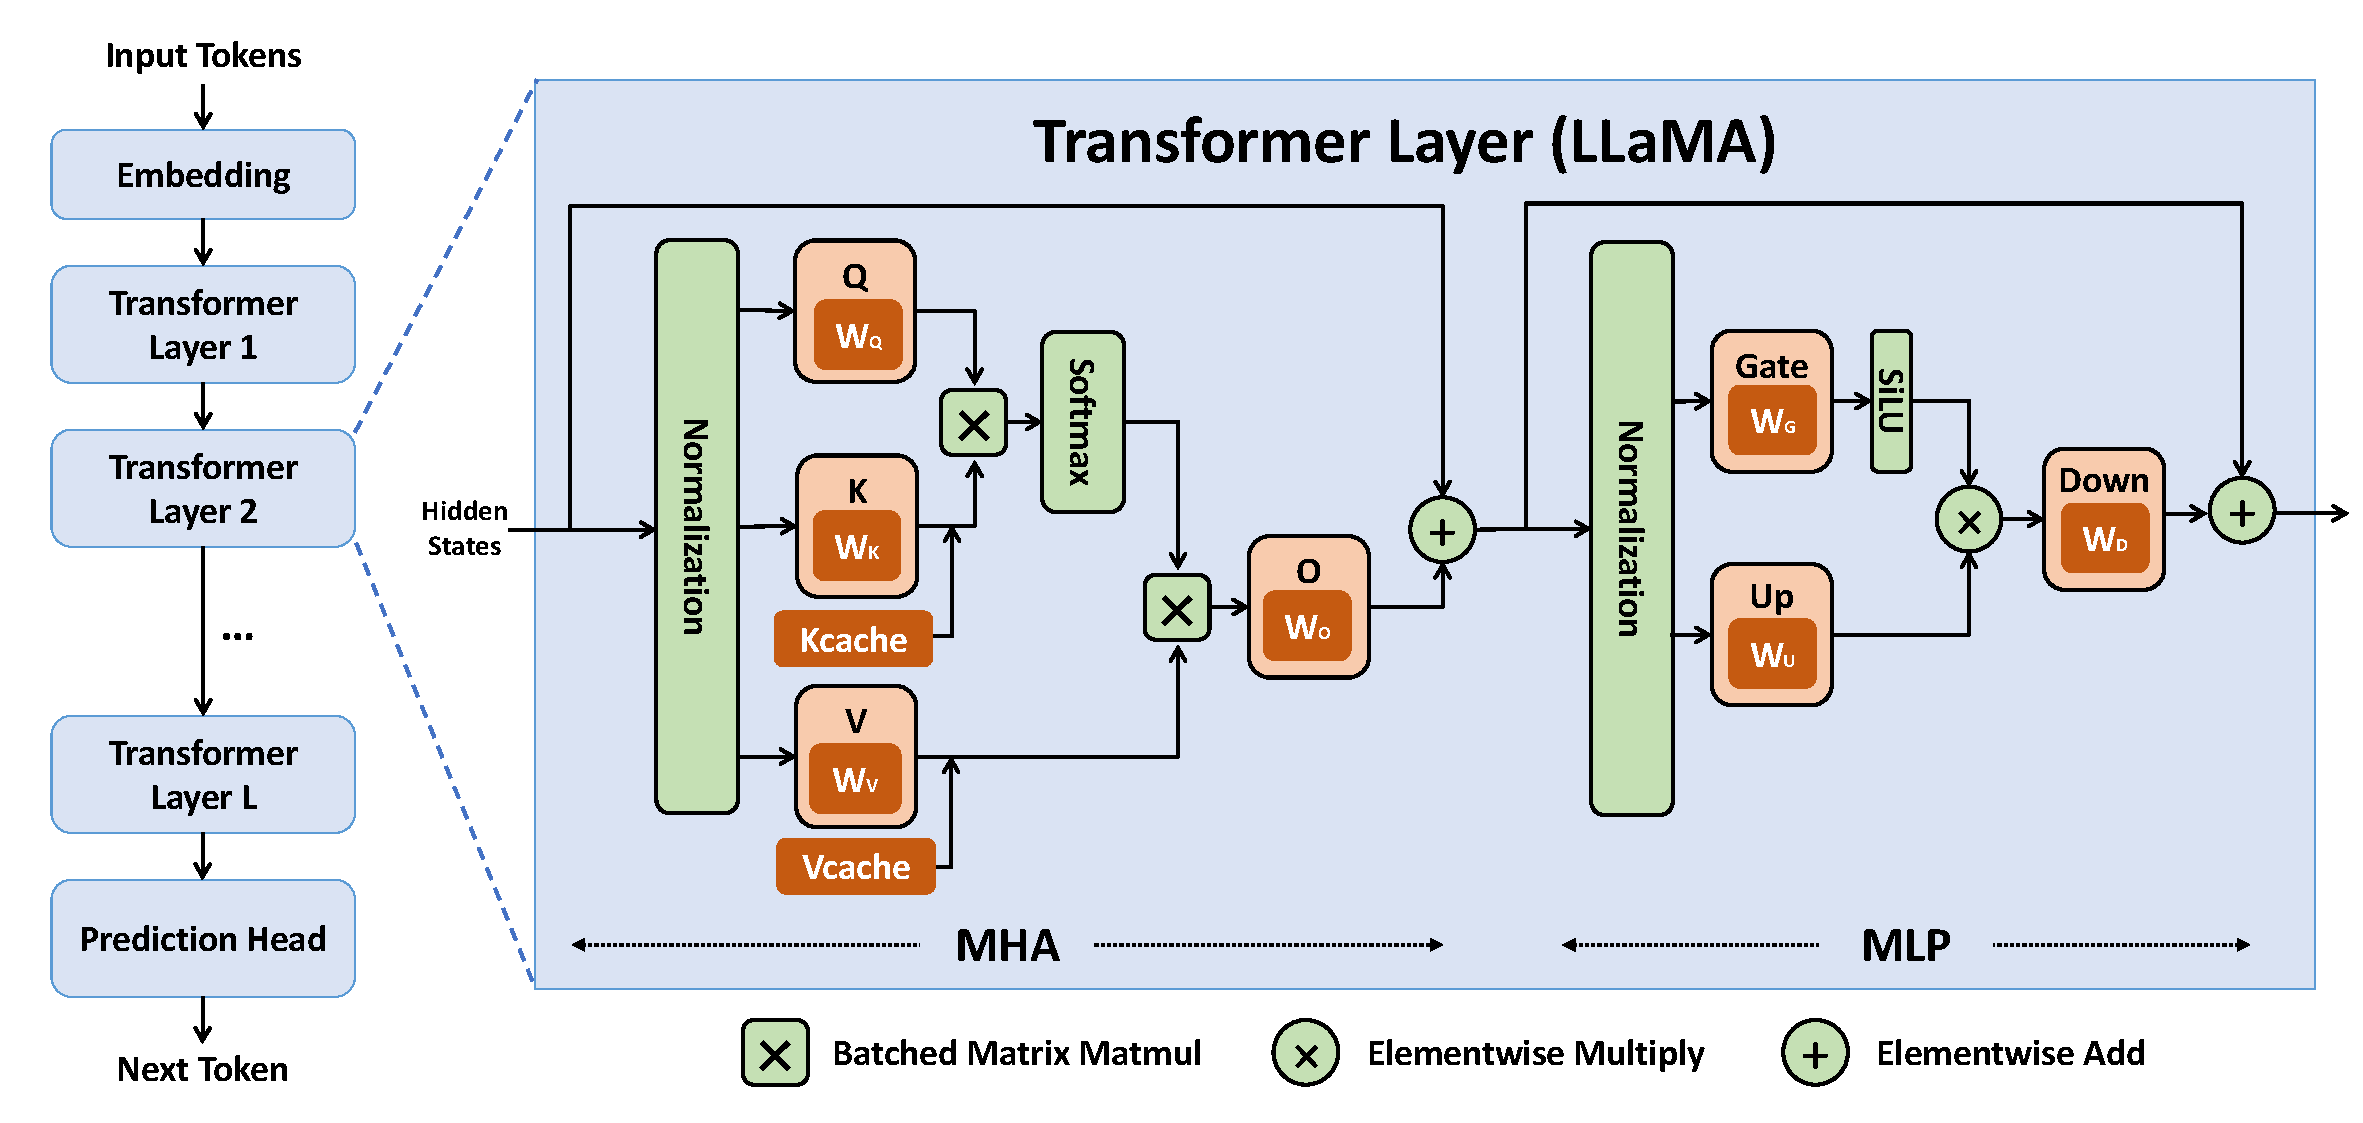
\includegraphics[width=0.8\linewidth]{ims/transformer_arch.pdf}
    \caption{LLM 架构示意图。}
    \label{fig:transformer_layer}
\end{figure*}

当前大多数大语言模型（LLM）采用 Transformer 解码器架构。
这里给出其基础结构概览，更深入内容可参考综述~\cite{zhao2023survey}。
该结构通常由 embedding 层、多层串联 Transformer 层和预测头组成，图~\ref{fig:transformer_layer} 给出了示意。

embedding 层将输入 token 映射为隐藏状态；隐藏状态进入 Transformer 层。
每个 Transformer 层通常由两部分组成：
首先是 masked multi-head attention（\textbf{MHA}），随后是 multi-layer perceptron（\textbf{MLP}）。
最后一层 Transformer 输出送入 prediction head，以预测下一个 token。

推理与训练相对：训练阶段模型通过数据更新参数；推理阶段参数固定，用户输入 \textbf{prompt}，模型生成 \textbf{response}。
LLM 推理通常分为两阶段：\textbf{Prefill} 与 \textbf{Decode}。

Prefill 是初始化阶段：模型接收 prompt 序列，并在每个 Transformer 层构建 key-value cache（KV cache），为后续生成打基础。

在 Prefill 中，MHA 计算并缓存 key/value。设某层输入为 $\mathbf{X}_{\text{pre}} \in \mathbb{R}^{n\times d}$，其中 $d$ 为隐藏维度，$n$ 为 prompt 长度；权重为 $\mathbf{W}_q,\mathbf{W}_k,\mathbf{W}_v,\mathbf{W}_o$。则：
\begin{align*}
\text{Query:} \quad \mathbf{Q}_{\text{pre}} &=  \mathbf{X}_{\text{pre}} \cdot \mathbf{W}_q \\
\text{Key:} \quad \mathbf{K}_{\text{pre}} &=  \mathbf{X}_{\text{pre}} \cdot \mathbf{W}_k \\
\text{Value:} \quad \mathbf{V}_{\text{pre}} &= \mathbf{X}_{\text{pre}} \cdot \mathbf{W}_v 
\end{align*}
$\mathbf{K}_{\text{pre}}$ 与 $\mathbf{V}_{\text{pre}}$ 被写入 KV cache。其余计算可写为\footnote{为简洁起见，省略 layer norm、position mask 与 positional embedding。}：
\begin{align*}
\mathbf{O}_{\text{pre}} &= \text{softmax}\left(\frac{\mathbf{Q}_{\text{pre}} \cdot \mathbf{K}_{\text{pre}}^T}{\sqrt{d}}\right) \cdot \mathbf{V}_{\text{pre}}\cdot \mathbf{W}_o +\mathbf{X}_{\text{pre}},
\end{align*}
其中 $\mathbf{O}_{\text{pre}} \in \mathbb{R}^{n\times d}$ 进入 MLP，MLP 输出作为下一层输入。

Decode 是核心生成阶段。模型读取并更新已缓存的 KV 信息，逐 token 生成输出；每个新 token 都依赖之前已生成 token。

在 Decode 中，MHA 读取 $\mathbf{K}_{\text{cache}},\mathbf{V}_{\text{cache}}$，输入为 $\mathbf{X}_{\text{dec}} \in \mathbb{R}^{1\times d}$，并拼接新 key/value：
\begin{align*}
\text{Query:} \quad \mathbf{Q}_{\text{dec}} &=  \mathbf{X}_{\text{dec}} \cdot \mathbf{W}_q \\
\text{Key:} \quad \mathbf{K}_{\text{cat}} &=  [\mathbf{K}_{\text{cache}}, \mathbf{X}_{\text{dec}} \cdot \mathbf{W}_k] \\
\text{Value:} \quad \mathbf{V}_{\text{cat}} &=  [\mathbf{V}_{\text{cache}}, \mathbf{X}_{\text{dec}} \cdot \mathbf{W}_v]
\end{align*}
并执行：
\begin{align*}
\mathbf{O}_{\text{dec}} &= \text{softmax}\left(\frac{\mathbf{Q}_{\text{dec}} \cdot \mathbf{K}_{\text{cat}}^T}{\sqrt{d}}\right) \cdot \mathbf{V}_{\text{cat}} \cdot \mathbf{W}_o + \mathbf{X}_{\text{dec}}
\end{align*}
其中 $\mathbf{O}_{\text{dec}} \in \mathbb{R}^{1\times d}$ 进入 MLP。最后一层输出送入预测头得到下一个 token。

\subsection{Roofline 模型}
\label{sec:Rooflinemodel}

评估 LLM 在特定硬件上的部署效率，需要同时考虑硬件特性与模型特性。
为此我们采用 Roofline 模型。
Roofline 是评估模型在目标硬件上理论性能上限的有效工具，可区分 memory bottleneck 与 compute bottleneck。

\begin{figure}[t]
    \centering
    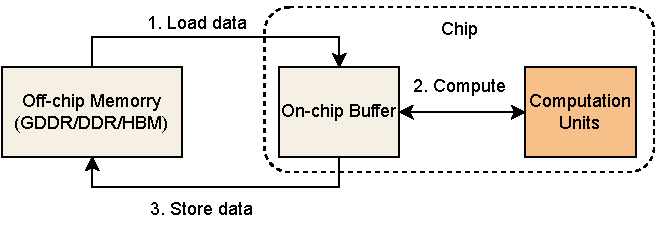
\includegraphics[width=0.95\linewidth]{ims/hardware_run.pdf}
    \caption{硬件上执行算子的过程。}
    \label{fig:hardware_run}
\end{figure}

如图~\ref{fig:hardware_run}，神经网络层执行包含：数据从 DDR/HBM 读入片上缓冲区，片上计算单元完成计算，再写回内存。
因此性能分析必须同时考虑内存访问与计算能力。
若某层计算量大、访存少，则是 compute-bound；反之访存重、计算轻，则是 memory-bound。
Roofline 能清晰区分二者并给出各场景性能上界。

\begin{figure}[t]
    \centering
    \includegraphics[width=0.95\linewidth]{ims/Roofline_nvidia_A6000.pdf}
    \caption{Nvidia A6000 的 Roofline 示意（FP16 计算）。}
    \label{fig:Roofline}
\end{figure}

使用 Roofline 主要两步：

1. \textbf{绘制 Roofline}：确定目标硬件峰值算力（OPS）与峰值带宽（bytes/s）\footnote{OPS 表示每秒操作数；一次 MAC 记为两次操作。}。
在坐标中以性能（OPS）为 y 轴、算术强度（OPs/byte）为 x 轴：
绘制峰值算力水平线（compute roof）与斜率为峰值带宽的对角线（memory roofline）。
图~\ref{fig:Roofline} 给出 A6000 示例。

2. \textbf{逐层分析}：统计各层 OPs 与内存访问字节数，计算算术强度（OPs/byte）。
再依据第一步图像读取理论性能上界，判断当前点是 memory-bound 还是 compute-bound，以指导后续优化策略。

\begin{table}[tb]
\caption{基于 Nvidia A6000 Roofline 对 Llama-2-7b 各层分析（序列长 2048，batch=1）。}
\label{tab:Llama_analysis}
\resizebox{\linewidth}{!}{
\begin{tabular}{@{}cccccc@{}}
\toprule
层名 & OPs  & \begin{tabular}[c]{@{}c@{}}内存\\访问\end{tabular} & \begin{tabular}[c]{@{}c@{}}算术\\强度\end{tabular} & \begin{tabular}[c]{@{}c@{}}最大\\性能\end{tabular} & 受限类型   \\ \midrule
\multicolumn{6}{c}{Prefill} \\ \midrule
q\_proj    & 69G  & 67M  & 1024 & 155T & compute \\
k\_proj    & 69G  & 67M  & 1024 & 155T & compute \\
v\_proj    & 69G  & 67M  & 1024 & 155T & compute \\
o\_proj    & 69G  & 67M  & 1024 & 155T & compute \\
gate\_proj & 185G & 152M & 1215 & 155T & compute \\
up\_proj   & 185G & 152M & 1215 & 155T & compute \\
down\_proj & 185G & 152M & 1215 & 155T & compute \\
qk\_matmul & 34G  & 302M & 114  & 87T  & memory  \\
sv\_matmul & 34G  & 302M & 114  & 87T  & memory  \\
softmax    & 671M & 537M & 1.25 & 960G & memory  \\
norm       & 59M  & 34M  & 1.75 & 1T   & memory  \\
add        & 8M   & 34M  & 0.25 & 192G & memory  \\ \midrule
\multicolumn{6}{c}{Decode} \\ \midrule
q\_proj    & 34M  & 34M  & 1    & 768G & memory  \\
k\_proj    & 34M  & 34M  & 1    & 768G & memory  \\
v\_proj    & 34M  & 34M  & 1    & 768G & memory  \\
o\_proj    & 34M  & 34M  & 1    & 768G & memory  \\
gate\_proj & 90M  & 90M  & 1    & 768G & memory  \\
up\_proj   & 90M  & 90M  & 1    & 768G & memory  \\
down\_proj & 90M  & 90M  & 1    & 768G & memory  \\
qk\_matmul & 17M  & 17M  & 0.99 & 762G & memory  \\
sv\_matmul & 17M  & 17M  & 0.99 & 762G & memory  \\
softmax    & 328K & 262K & 1.25 & 960G & memory  \\
norm       & 29K  & 16K  & 1.75 & 1T   & memory  \\
add        & 4K   & 16K  & 0.25 & 192G & memory  \\ \bottomrule
\end{tabular}
}
\end{table}

资源未被充分利用通常有两类情况：
当算术强度低于拐点（红区）时，单位访存对应计算量小，即便带宽打满也无法吃满算力，此时为 memory-bound，可优先采用量化、算子融合、增大 batch 等方法缓解访存压力。
当算术强度高于拐点（绿区）时，少量访存即可触发大量计算，此时为 compute-bound，可考虑低比特计算等方式提升计算效率。

以表~\ref{tab:Llama_analysis} 为例，Llama-2-7b 在 A6000 上 prefill 多为 compute-bound、性能较高；decode 全部 memory-bound，性能显著低于 GPU 峰值算力。
在交互式场景中 prefill 仅执行一次，而 decode 会反复执行生成连续输出，因此 decode 的 memory-bound 优化是大模型推理加速的核心。

\subsection{LLM-Viewer}
\label{sec:llmviewer}

LLM 由多层 Transformer 组成，每层操作类型复杂，且不同模型操作组合并不一致。
同时还需追踪 memory footprint 以估计峰值显存与总推理时延。
因此，LLM 分析必须是“网络级”分析而非单算子分析。

我们提出 LLM-Viewer\footnote{工具开源于 https://github.com/hahnyuan/LLM-Viewer} 进行网络级分析。
它支持在多种硬件平台上分析 LLM 性能与效率，为推理优化提供可解释依据。

LLM-Viewer 工作流（图~\ref{fig:llmviewer_workflow}）包括：
(1) 输入 LLM，提取各层计算量、输入输出张量形状和数据依赖；
(2) 输入硬件参数，构建对应 Roofline 模型（算力与带宽）；
(3) 设置推理配置，如 batch size、prompt 长度、生成长度；
(4) 设置优化配置，如量化比特、是否使用 FlashAttention、解码策略和系统优化；
(5) Analyzer 基于 Roofline 与层级信息评估逐层性能，并按数据依赖追踪内存占用，得到峰值内存和整网性能；
(6) 生成报告，给出各层与整网性能上界、瓶颈与内存占用，可进一步绘制 batch-size/sequence-length 等分析曲线；
(7) 提供 Web 可视化界面，便于配置调整与逐层结果查看。
